\section{Besonderheiten von Vektoruhren}

Nach Betrachtung der Funktionsweise von Vektoruhren sowie einer Beschreibung von besonderen Problemen, gibt es noch weiterführende Aspekte zu beachten. 
TODO: Mehr text hier! 
\subsection{Causaly Ordered Multicast}

In einem Verteilten System kann es recht schnell passieren, dass sich die Reihenfolge von gesendeten Broadcasts bei dem Empfänger und dem Sender unterscheiden. Dies führt in gewissen Fällen zu Problemen, wenn z.B. die Daten eines zweiten Broadcast von denen des ersten abhängen, es also eine temporale korrelation gibt. Um diesen Problem zu lösen, haben Kenneth P. Birman und Thomas A. Joseph in \cite{Birman:1987:RCP:7351.7478} den sogenannten Causal Brooadcast eingeführt, welcher auch als Causaly Ordered Multicast bezeichnet werden kann.

Wie in \cite{Birman:1987:RCP:7351.7478}[S. 52, Kapitel 3.3] beschrieben, kann es vorkommen, dass sich die Reihenfolge der gesendeten Nachrichten eines Senders und die Reihenfolge der empfangenen Nachrichten am Empfänger unterscheiden. Dies kann etwa durch Verzögerungen auf dem Übertragungsweg geschehen. Bei einem herkömmlichen Broadcast, welcher in einem System mit Vektoruhren abgesendet wird, ist kein Mechanismus vorgesehen, um eine eventuell für die Funktionsweise der Anwendung notwendige Reihenfolge der versendeten Nachrichten einzuhalten. Die Broadcast-Nachricht wird einfach an alle Teilnehmer versendet und nicht weiter beachtet.

Anders ist dies bei einem Causaly Orderen Multicast. Wie der Name bereit vermuten lässt, spielt hierbei die Ordnung der Multicasts nach deren Kausalität, also der Ursache eine Rolle. Die Ursache ist in diesem Fall das Verschicken des Broadcast am Sender. Somit werden bei einem Causal Broadcast die Nachrichten nach deren Reihenfolge des Versendens am Empfängerprozess geordnet. Um eine Rückantwort eines jeden Nodes an den Sender mit einer Empfangsbestätigung zu vermeiden, kann ein Causally Ordered Multicast auf Basis der Vektoruhren in den Empfängern umgesetzt werden. Durch die Vektoruhr kann ein Node entscheiden, ob er bei Empfang einer Nachricht alle Broadcast des entsprechenden Senders erhalten hat, die in der kausalen Vergangenheit dieses Broadcasts empfangen hat. Ist dies nicht der Fall, muss er die Nachricht in eine Warteliste setzten und diese erst annehmen, sobald alle in der Zwischenzeit passierten Broadcasts angekommen sind. Abbildung \ref{figure:causalbroadcast} verdeutlicht diese Funktionsweise genauer.

\begin{figure}[ht]
	\centering
	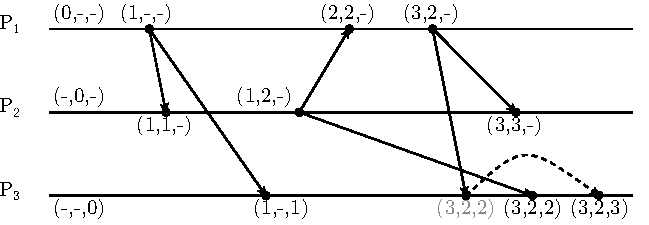
\includegraphics[width=10cm]{kommBeispielCausalBroadcast.pdf}
	\caption[Kommunikation durch Causally Ordered Multicasts]{Ablauf einer Kommunikation zwischen Prozessen, die ausschließlich Causally Ordered Multicasts versenden. Wie man sieht, muss ein Prozess eine Empfangene Nachricht aufheben, bis eine vorher gesendete Nachricht eintrifft.}
	\label{figure:causalbroadcast}
\end{figure}
\FloatBarrier

Der Ablauf des Aufhebens und Verzögerns von gewissen Nachrichten lässt sich durch ein recht einfaches Protokoll darstellen. Dieses ist in Abbildung \ref{figure:causalBroadcastProtocol} dargestellt.

\begin{figure}[ht]
	\centering
	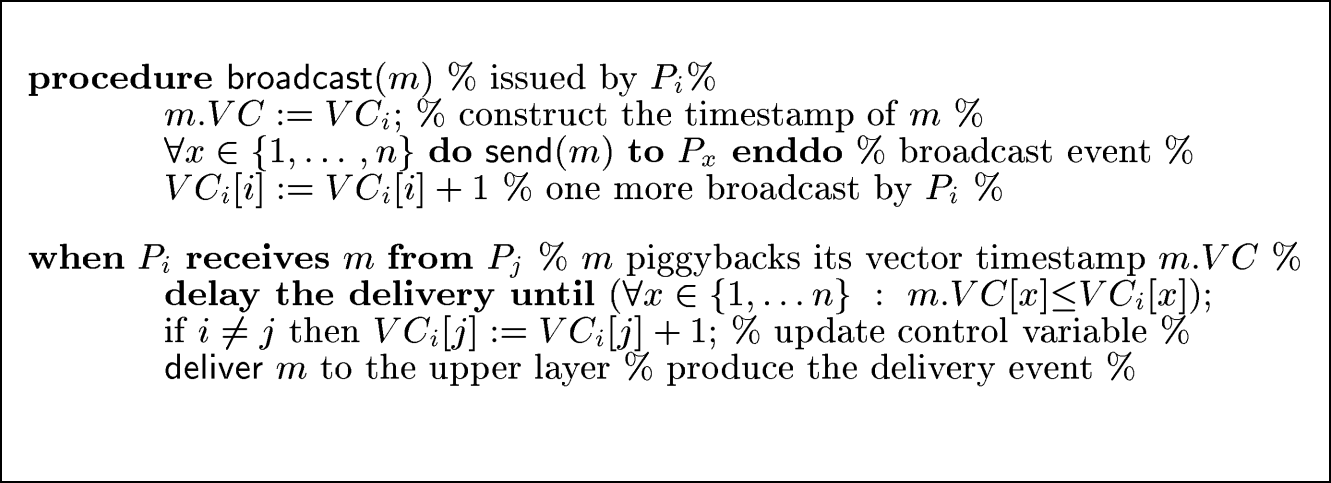
\includegraphics[width=10cm]{causalBroadcastProtocol.png}
	\caption[Protokoll für den Causally Ordered Multicast]{Beschreibung der verarbeitung von Causally Ordered Multicast in Form eines Protokolls.}
	Quelle: \cite{Baldoni:2002:FDC:1435723.1437765}[S. 7, Abbildung 3]
	\label{figure:causalBroadcastProtocol}
\end{figure}
\FloatBarrier

Ausgeschrieben sieht die Funktionalität des Protokolls folgendermaßen aus:

\begin{itemize}
	\item Löst ein Prozess durch ein stattgefundenes Event einen Broadcast aus, so fügt er zunächst seine aktuelle Vektoruhr an die Nachricht des Broadcasts an. Nun sendet er die Nachricht an alle teilnehmenden Prozesse und aktualisiert im letzten Schritt seinen Eintrag in der lokalen Vektoruhr.
	\item Empfängt ein Prozess $P_i$ eine Nachricht m des Prozesses $P_j$, so muss er die Nachricht so lange verzögern, bis die Bedingung $m.VC[x] \le VC_i[x]$ erfüllt ist, also bis die Nachricht ein direkter Nachfolger der Vorherigen ist. Anschließend wird der wert VC[j] inkrementiert, um das Sendeevent des Prozesses $P_j$ zu verzeichnen. Nun kann die Nachricht an die Anwendungsschicht weitergegeben werden.
\end{itemize}

Im Laufe der Kommunikation kann es passieren, dass mehrere nacheinander empfangenen Nachrichten nicht sofort verwendet sondern verzögert werden müssen. Für diesen Fall bietet es sich an, die verzögerten Nachrichten in einer liste zu speichern und bei Eintreffen einer Neuen Nachricht alle zunächst zurückgehaltenen nach deren \qq{alter} zu verarbeiten.

\subsubsection{Umsetzung in C\# auf Basis der Vektoruhr}
Causaly Ordered Multicasts wurden als Erweiterung der in Kapitel \ref{vectorClockImpl} beschriebenen Implementierung eingefügt. In dem gewählten Bank-Szenario sendet ein Bankautomat bei jeder Kontoaktualisierung, also einem Event, einen Broadcast an alle im System vorhandenen Prozesse. Dabei ist es jedoch egal ob die gesendeten Nachrichten über die Aktualisierung auch ankommen oder nicht beziehungsweise spielt die Reihenfolge des Empfangs für den Sender keine Rolle. Dieses System funktioniert solange, bis ein Prozess einmal eine Aktualisierung zu spät erhält und somit seinen Kontostand nicht entsprechend zum richtigen Zeitpunkt aktualisiert. Um diesem Problem entgegenzuwirken, können Causal Broadcasts helfen.

Als Grundlage dient die in Kapitel \ref{vectorClockImpl} implementierte Vektoruhren-Mechanik. Jedoch gibt es einige Unterschiede bei der Aktualisierung der Uhren beziehungsweise des Zeitpunkts der Aktualisierung.


 
\subsection{Rolle der Anwendungsschicht (Anwendungs-API)}
\label{RolleDerAnwendung}